%% ===================================================================================
%% Undergraduate Thesis Template using abntex2
%% Version: 1.0
%% Based on the original abntex2 model by the abnTeX2 group and derivatives.
%% This template is designed to be a clean, modern, and easy-to-use starting
%% point for undergraduate theses, following ABNT standards.
%% ===================================================================================

% Use the new 'freelance-doc' class
\documentclass[
	% -- Memoir Class Options --
	12pt,% Font size
	openright,% Chapters start on odd-numbered pages
	oneside,% For single-sided printing
	a4paper,% Paper size
	% -- Babel Package Options --
	english,% Additional language for hyphenation
	brazil% Main document language
]{freelance-doc}

%% ===================================================================================
%% PACKAGE IMPORTS
%% ===================================================================================

% -----------------------------------------------------------------------------------
% -- Fundamental Packages
% -----------------------------------------------------------------------------------
\usepackage[T1]{fontenc}      % Use 8-bit T1 fonts
\usepackage[utf8]{inputenc}   % UTF-8 input encoding for accents and special characters
\usepackage{lmodern}          % Use the Latin Modern font family for better PDF rendering
\usepackage{indentfirst}      % Indent the first paragraph of each section
\usepackage{cmap}             % Make the PDF searchable and copyable

% -----------------------------------------------------------------------------------
% -- Graphics and Colors
% -----------------------------------------------------------------------------------
\usepackage{graphicx}         % For including images
% \usepackage{xcolor}           % Already being added
\usepackage{subcaption}       % For creating subfigures within a figure environment

% -----------------------------------------------------------------------------------
% -- Tables and Listings
% -----------------------------------------------------------------------------------
\usepackage{booktabs}         % For professional-quality tables
\usepackage{listings}         % For basic code listings
\usepackage{minted}           % For advanced, syntax-highlighted code listings (requires Python's Pygments)
% \usepackage[table]{xcolor}    % To add color to table rows/cells
\usepackage{multirow}         % For 
% -----------------------------------------------------------------------------------
% -- Mathematics
% -----------------------------------------------------------------------------------
\usepackage{amsmath, amsfonts, amssymb} % For advanced math typesetting

% -----------------------------------------------------------------------------------
% -- Code Formating
% --------------------------------------------------------------------------------------
\usepackage{inconsolata} % or try \usepackage{inconsolata} or \usepackage{FiraMono}
\lstset{
    numbers=left,
    numberstyle=\tiny,
    numbersep=8pt,                  % Space between line numbers and code
    frame=single,                   % Box around code
    framesep=6pt,                   % Space between frame and code
    xleftmargin=2em,                % Indent code block to fit line numbers
    xrightmargin=1em,
    breaklines=true,
    postbreak=\mbox{$\hookrightarrow$\space},
    basicstyle=\linespread{1.05}\ttfamily\footnotesize, % Use better mono font and size
    keywordstyle=,
    commentstyle=,
    stringstyle=,
    showstringspaces=false,
    tabsize=2,
    captionpos=b,
    rulecolor=,
}
% -----------------------------------------------------------------------------------
% -- Citation and Bibliography
% -----------------------------------------------------------------------------------
\usepackage[num]{abntex2cite}  % ABNT compliant citation style (numeric)
% For author-date style, use: \usepackage[alf]{abntex2cite}

%% ===================================================================================
%% CUSTOM COMMANDS AND CONFIGURATIONS
%% ===================================================================================

%% ===================================================================================
%% DOCUMENT INFORMATION (Updated for Freelance Work)
%% ===================================================================================

% [TODO: Fill in your project information here]
\titulo{Grana Livre}
\autor{Caio Reis (Desenvolvedor e Mantenedor do Projeto) \and Felipe (Desenvolvedor) \and Gabriel (Desenvolvedor) \and Silviano (Desenvolvedor)}
\cliente{}
\local{City, State}
\data{\the\year}
\newcommand{\urlrepositorio}{https://github.com/fromcaio/tec-web}

% --- Images for the Cover Page ---
% [TODO: Make sure these image files exist in the 'imgs' folder]
\toplogo{imgs/cover-top.png}
\bottomlogo{imgs/cover-bottom.png}
\closingimage{imgs/closing-image.png} % <-- ADD THIS LINE
% -----------------------------------------------------------------------------------
% -- PDF Hyperlinks and Metadata Configuration
% -----------------------------------------------------------------------------------
\definecolor{hyperlinkblue}{RGB}{41, 5, 195} % Custom blue for links

\makeatletter
\hypersetup{
    pdftitle={\@title},
    pdfauthor={\@author},
    pdfsubject={\imprimirpreambulo},
    pdfcreator={LaTeX with abnTeX2},
    pdfkeywords={keyword1}{keyword2}{keyword3},
    colorlinks=true,
    linkcolor=hyperlinkblue,
    citecolor=hyperlinkblue,
    filecolor=magenta,
    urlcolor=hyperlinkblue,
    bookmarksdepth=4,
    bookmarkstype=toc
}
\makeatother

% -----------------------------------------------------------------------------------
% -- Spacing and Layout
% -----------------------------------------------------------------------------------
\setlength{\parindent}{1.5cm} % Paragraph indentation
\setlength{\parskip}{0.2cm}   % Vertical space between paragraphs

% -----------------------------------------------------------------------------------
% -- Indexing
% -----------------------------------------------------------------------------------
\makeindex % Generate the index file

%% ===================================================================================
%% DOCUMENT START
%% ===================================================================================
\begin{document}

% Use Brazilian Portuguese hyphenation patterns and spacing rules
\frenchspacing

% ----------------------------------------------------------
% -- PRE-TEXTUAL ELEMENTS
% ----------------------------------------------------------
\pretextual

% --- Cover and Title Page ---
% \imprimircapa
\imprimircapalogo
\imprimirfolhaderosto

% --- Other pre-textual elements (Approval page, Dedication, etc.) are in a separate file ---
% [TODO: Edit the 'pretextual_elements.tex' file with your information]
%% ===================================================================================
%% Pre-Textual Elements (pretextual_elements.tex)
%% Version: 2.0 (Freelance)
%%
%% This file contains the Executive Summary for the project deliverable.
%% ===================================================================================


% -----------------------------------------------------------------------------------
% -- EXECUTIVE SUMMARY (Sumário Executivo)
% -----------------------------------------------------------------------------------
% This section provides a high-level overview of the project document.
% -----------------------------------------------------------------------------------
\begin{resumo}[Resumo]

  % [TODO: Write the executive summary of your project here.]
  This summary should briefly describe the project's objectives, the scope of the work delivered, the key outcomes, and any major conclusions or recommendations. It is intended for stakeholders who need a quick understanding of the document's contents without reading it in its entirety. It should be written in a single paragraph.

  \vspace{\onelineskip} % Adds a blank line before the keywords
  \noindent % Prevents indentation for the keywords line
  \textbf{Palavras-chave}: tecnologia-chave; entregável-principal; nome-do-projeto.
\end{resumo}


% -----------------------------------------------------------------------------------
% -- The following academic sections have been removed for the freelance template:
% -- Folha de Aprovação (Approval Sheet)
% -- Dedicatória (Dedication)
% -- Agradecimentos (Acknowledgements)
% -- Epígrafe (Epigraph)
% -- Abstract (Second language abstract)
% -----------------------------------------------------------------------------------

% --- List of Figures ---
\pdfbookmark[0]{\listfigurename}{lof}
\listoffigures*
\cleardoublepage

% --- List of Tables (Optional) ---
% [TODO: Uncomment the following lines if your thesis contains tables]
\pdfbookmark[0]{\listtablename}{lot}
\listoftables*
\cleardoublepage

% --- List of Acronyms and Abbreviations ---
% [TODO: Add your acronyms to the 'acronyms.tex' file and uncomment below]
% %% ===================================================================================
%% Acronyms and Abbreviations (acronyms.tex)
%%
%% This file contains the list of acronyms used in the thesis.
%%
%% To use this file:
%% 1. Add your acronyms below following the example format.
%% 2. In main.tex, uncomment the line that reads: %% ===================================================================================
%% Acronyms and Abbreviations (acronyms.tex)
%%
%% This file contains the list of acronyms used in the thesis.
%%
%% To use this file:
%% 1. Add your acronyms below following the example format.
%% 2. In main.tex, uncomment the line that reads: %% ===================================================================================
%% Acronyms and Abbreviations (acronyms.tex)
%%
%% This file contains the list of acronyms used in the thesis.
%%
%% To use this file:
%% 1. Add your acronyms below following the example format.
%% 2. In main.tex, uncomment the line that reads: \include{acronyms}
%% ===================================================================================

% The 'siglas' environment creates the list of acronyms.
\begin{siglas}
	% [TODO: Add your project's acronyms and abbreviations here.]
	% The format is: \item[ACRONYM] Full Name / Description
	
	\item[ABNT] Associação Brasileira de Normas Técnicas
	\item[API] Application Programming Interface
	\item[CPU] Central Processing Unit
	\item[HTML] HyperText Markup Language
	\item[IDE] Integrated Development Environment
	\item[JSON] JavaScript Object Notation
	\item[SQL] Structured Query Language
	
\end{siglas}
%% ===================================================================================

% The 'siglas' environment creates the list of acronyms.
\begin{siglas}
	% [TODO: Add your project's acronyms and abbreviations here.]
	% The format is: \item[ACRONYM] Full Name / Description
	
	\item[ABNT] Associação Brasileira de Normas Técnicas
	\item[API] Application Programming Interface
	\item[CPU] Central Processing Unit
	\item[HTML] HyperText Markup Language
	\item[IDE] Integrated Development Environment
	\item[JSON] JavaScript Object Notation
	\item[SQL] Structured Query Language
	
\end{siglas}
%% ===================================================================================

% The 'siglas' environment creates the list of acronyms.
\begin{siglas}
	% [TODO: Add your project's acronyms and abbreviations here.]
	% The format is: \item[ACRONYM] Full Name / Description
	
	\item[ABNT] Associação Brasileira de Normas Técnicas
	\item[API] Application Programming Interface
	\item[CPU] Central Processing Unit
	\item[HTML] HyperText Markup Language
	\item[IDE] Integrated Development Environment
	\item[JSON] JavaScript Object Notation
	\item[SQL] Structured Query Language
	
\end{siglas}

% --- List of Symbols (Optional) ---
% [TODO: Uncomment if you have a list of symbols]
\begin{simbolos}
   \item[$ \alpha $] -- Description of alpha symbol.
   \item[$ \beta $] -- Description of beta symbol.
\end{simbolos}
\cleardoublepage

% --- Table of Contents ---
\pdfbookmark[0]{\contentsname}{toc}
\tableofcontents*
\cleardoublepage

% ----------------------------------------------------------
% -- TEXTUAL ELEMENTS (CHAPTERS)
% ----------------------------------------------------------
\textual

% [TODO: Write your chapters in these separate .tex files]
% This modular approach is highly recommended for managing large documents.
\chapter{Introdução}\label{cap:intro}

\section{Contextualização}
O controle financeiro pessoal é uma prática essencial para o equilíbrio das finanças de qualquer indivíduo. Apesar disso, muitas pessoas ainda encontram dificuldades em organizar receitas, despesas e investimentos de forma clara e acessível. Nesse cenário, surgem ferramentas digitais que auxiliam na gestão financeira, mas grande parte delas é paga, possui funcionalidades gratuitas limitadas ou não oferece transparência no uso dos dados. E em sua grande maioria, essas soluções são desenvolvidas no exterior, não considerando as especificidades da realidade financeira brasileira, como métodos de pagamento locais, moedas regionais ou particularidades do sistema bancário nacional.

Com base nessa necessidade, o projeto \textit{GranaLivre} foi idealizado como uma plataforma \textit{open source} voltada para o gerenciamento de finanças pessoais, desenvolvida por brasileiros e para brasileiros. Seu propósito é oferecer uma solução simples, intuitiva e acessível, que valorize a cultura nacional e atenda às demandas específicas do público brasileiro, permitindo que qualquer usuário tenha maior controle sobre suas finanças sem depender de sistemas proprietários estrangeiros. O projeto busca fortalecer a comunidade de desenvolvedores brasileiros, oferecendo uma base tecnológica sólida e totalmente documentada em português, incentivando a participação ativa da comunidade local no desenvolvimento e evolução contínua da plataforma.

\section{Motivação}
A motivação para o desenvolvimento do \textit{GranaLivre} está diretamente ligada à importância da autonomia financeira e à democratização do acesso a ferramentas de planejamento. Além disso, muitas soluções existentes são documentadas apenas em inglês, o que dificulta a participação de desenvolvedores brasileiros. O \textit{GranaLivre}, ao disponibilizar toda a documentação em português, busca valorizar a comunidade local e ampliar as oportunidades de contribuição, considerando a cultura e as necessidades específicas do público brasileiro.

\section{Objetivos}

\subsection{Objetivo Geral}
Desenvolver uma aplicação web de finanças pessoais que permita aos usuários organizar receitas, despesas, investimentos e patrimônio de forma simples e intuitiva.

\subsection{Objetivos Específicos}
\begin{itemize}
    \item Disponibilizar uma plataforma \textit{open source}, gratuita e acessível a qualquer usuário;
    \item Permitir o registro e acompanhamento de receitas e despesas;
    \item Facilitar a gestão de contas recorrentes, assinaturas e metas financeiras;
    \item Oferecer visualização clara do saldo disponível e do patrimônio acumulado;
    \item Produzir documentação em português para engajar a comunidade de desenvolvedores brasileiros;
    \item Estabelecer uma base sólida para futuras evoluções do sistema, integrando recursos mais avançados de planejamento financeiro.
\end{itemize}

\section{Justificativa}
A justificativa do \textit{GranaLivre} está na necessidade crescente de ferramentas confiáveis, acessíveis e abertas para controle financeiro. Ao adotar o modelo \textit{open source}, o projeto garante não apenas a transparência no uso dos dados, mas também a possibilidade de evolução contínua por meio da colaboração da comunidade. Outro diferencial está na produção de documentação totalmente em português, o que reduz barreiras de entrada e valoriza a cultura local, permitindo que desenvolvedores brasileiros tenham maior facilidade para participar ativamente da evolução da plataforma. Assim, busca-se construir um sistema que ajude os usuários a alcançar maior organização e independência financeira.
\chapter{Fundamentação Teórica}\label{cap:fund_teorica}

\section{Conceitos Gerais}

O desenvolvimento de sistemas web modernos envolve a integração de múltiplas camadas e tecnologias, que vão desde a interface do usuário até a lógica de negócio e a persistência de dados. O projeto \textit{GranaLivre} adota uma arquitetura baseada na separação entre \textit{front-end} e \textit{back-end}, de modo a facilitar a escalabilidade, a colaboração entre desenvolvedores e a manutenção do sistema.

\section{Tecnologias Utilizadas}

\subsection{HTML, CSS e JavaScript}
A base do desenvolvimento \textit{front-end} é composta por HTML, CSS e JavaScript, tecnologias fundamentais para a construção de páginas web.  
O HTML organiza o conteúdo e define a estrutura semântica da aplicação, enquanto o CSS gerencia a aparência visual. Já o JavaScript possibilita a interação dinâmica e o controle dos componentes da interface, tornando a aplicação mais responsiva e intuitiva para o usuário.

\subsection{Next.js}
O \textit{Next.js} é um framework baseado em React que fornece uma estrutura organizada para o desenvolvimento de interfaces modernas.  
A escolha do Next.js justifica-se pela clareza no desenvolvimento, pela facilidade de criação de componentes reutilizáveis e pela boa integração com o ecossistema JavaScript.

\subsection{Node.js}
O \textit{Node.js} é utilizado como ambiente de execução do Next.js, permitindo que o código JavaScript seja processado no lado do servidor quando necessário. Essa tecnologia é fundamental para lidar com operações assíncronas e de alta performance, garantindo maior flexibilidade ao front-end.

\subsection{Python e Django}
O \textit{back-end} do sistema é desenvolvido em Python, utilizando o framework \textit{Django}. Esse framework fornece uma estrutura robusta para o desenvolvimento rápido de aplicações web, oferecendo recursos nativos como sistema de autenticação, gerenciamento de banco de dados via ORM e uma arquitetura organizada em padrões de projeto.  
O Django foi escolhido por sua maturidade, comunidade ativa e facilidade de integração com diferentes bancos de dados relacionais.

\subsection{SQLite}
O banco de dados escolhido para o projeto é o \textit{SQLite}, um sistema de gerenciamento de banco de dados relacional (RDBMS) \textit{serverless} (sem servidor). Sua principal vantagem reside na leveza e simplicidade, armazenando todo o banco de dados em um único arquivo no sistema de arquivos. Esta escolha é estratégica para o \textit{GranaLivre} por diversos motivos:
\begin{itemize}
    \item \textbf{Execução Local e Portabilidade:} Por não requerer um processo de servidor separado, o SQLite é ideal para aplicações onde o usuário executa o software localmente, eliminando a complexidade de gerenciar uma instância de banco de dados externa. Isso também facilita a implementação de futuras versões desktop, onde a base de dados pode ser facilmente empacotada com a aplicação.
    \item \textbf{Facilidade na Geração de Instaladores:} Ao empacotar a aplicação, o arquivo do banco de dados SQLite pode ser incluído diretamente, resultando em instaladores mais leves e fáceis de distribuir, sem a necessidade de configurar um banco de dados complexo no ambiente do usuário.
    \item \textbf{Desenvolvimento Simplificado:} A integração com o ORM do Django é transparente e a manutenção da camada de persistência de dados se torna mais direta, pois não há dependências de serviços de banco de dados externos durante o desenvolvimento.
    \item \textbf{Desempenho para Aplicações de Usuário Único:} Para o perfil de uso do \textit{GranaLivre}, que foca no controle financeiro pessoal e geralmente opera em modo de usuário único, o desempenho do SQLite é mais do que adequado e eficiente.
\end{itemize}
A compatibilidade nativa do Django com SQLite facilita seu uso e manutenção, tornando-o uma escolha robusta para as necessidades atuais e futuras do projeto.

\subsection{Docker}
Para simplificar o processo de desenvolvimento, implantação e utilização do sistema, será utilizado o \textit{Docker}. Essa tecnologia permite a criação de ambientes isolados e padronizados, garantindo que a aplicação possa ser executada de maneira consistente em diferentes máquinas e servidores.  
Com isso, tanto desenvolvedores quanto usuários finais terão maior facilidade em instalar e utilizar o \textit{GranaLivre}.

\subsection{Git e GitHub}
O Git é um sistema de controle de versão distribuído, criado para gerenciar o histórico de alterações em projetos de software. Ele permite que múltiplos desenvolvedores trabalhem de forma colaborativa, rastreando cada modificação no código-fonte, facilitando a reversão de erros e permitindo a criação de ramificações (\textit{branches}) para o desenvolvimento de novas funcionalidades sem afetar a versão principal do projeto.

O GitHub, por sua vez, é uma plataforma de hospedagem de código-fonte que utiliza o Git como seu principal sistema de controle de versão. Ele funciona não apenas como um repositório remoto, mas como um centro de colaboração para projetos de software, especialmente os de código aberto.

No contexto do projeto \textit{GranaLivre}, o uso de Git e GitHub é fundamental por diversas razões:
\begin{itemize}
\item \textbf{Controle de Versão:} Todo o histórico de desenvolvimento do projeto será rastreado, garantindo segurança e organização.
\item \textbf{Colaboração Aberta:} O GitHub permite que qualquer desenvolvedor da comunidade possa "forkar" (criar uma cópia) o repositório, implementar melhorias e submeter suas contribuições através de \textit{Pull Requests}, que serão revisadas antes de serem integradas ao código principal.
\item \textbf{Gerenciamento do Projeto:} A plataforma oferece ferramentas como \textit{Issues} (para relatar bugs e sugerir novas funcionalidades) e \textit{Projects} (para organizar o fluxo de trabalho), centralizando a comunicação e o planejamento das tarefas.
\item \textbf{Divulgação e Transparência:} Manter o código-fonte em um repositório público no GitHub serve como o principal "cartão de visita" do projeto, atraindo novos colaboradores e garantindo total transparência sobre o funcionamento do sistema. O repositório do \textit{GranaLivre} pode ser acessado em: \url{\urlrepositorio}.
\end{itemize}
Dessa forma, o GitHub não é apenas uma ferramenta de desenvolvimento, mas também o principal ponto de encontro da comunidade em torno do \textit{GranaLivre}.

\section{Arquitetura Geral}
O sistema segue um modelo baseado na separação entre \textit{front-end} e \textit{back-end}. O \textit{front-end}, desenvolvido com Next.js, é responsável pela interface do usuário e comunicação com a API. Já o \textit{back-end}, construído em Django, expõe serviços e gerencia a persistência dos dados em PostgreSQL.  
O uso do Docker garante que toda essa arquitetura seja facilmente replicável e portável, favorecendo tanto o desenvolvimento colaborativo quanto a implantação.

\section{Trabalhos Relacionados}

Existem diversas aplicações de controle financeiro já disponíveis, tanto em formato proprietário quanto em projetos de código aberto. No entanto, muitas dessas soluções encontram-se em estágios avançados de desenvolvimento, com arquiteturas complexas e documentação predominantemente em inglês, o que pode dificultar a participação de novos colaboradores — especialmente estudantes e desenvolvedores brasileiros em formação.

O diferencial do \textit{GranaLivre} não está apenas em sua proposta funcional, mas sobretudo em seu caráter formativo e comunitário. O sistema foi concebido como uma aplicação em estágio inicial, organizada desde o início com boas práticas de desenvolvimento e documentação em português. Dessa forma, busca-se criar um ambiente convidativo para que desenvolvedores brasileiros possam contribuir ativamente, aprendendo e crescendo junto ao projeto.

A intenção é, portanto, não apenas oferecer uma alternativa de software de finanças pessoais, mas também construir um espaço colaborativo que valorize a cultura local, promova a troca de conhecimento e incentive a participação da comunidade no ecossistema de software livre.
\chapter{Metodologia}\label{cap:metodologia}

O desenvolvimento da plataforma \textit{GranaLivre} segue uma abordagem iterativa e incremental, organizada em quatro \textit{sprints} com duração aproximada de três semanas cada. Essa estrutura busca garantir entregas contínuas, com ciclos curtos de planejamento, implementação e validação. O cronograma definido contempla as seguintes entregas:

\begin{itemize}
    \item \textbf{Sprint 1}: 23/09/2025
    \item \textbf{Sprint 2}: 21/10/2025
    \item \textbf{Sprint 3}: 11/11/2025
    \item \textbf{Sprint 4}: 09/12/2025
\end{itemize}

\section{Sprint 1: Organização e Estruturação}

O primeiro ciclo concentrou-se na preparação do ambiente e na definição de diretrizes para todo o projeto. As principais atividades realizadas foram:

\begin{itemize}
    \item Estruturação da documentação inicial.
    \item Organização do repositório no GitHub, incluindo definição de \textit{branching model} e fluxo de trabalho.
    \item Definição de papéis da equipe.
    \item Elaboração de um diagrama de casos de uso.
    \item Modelagem do banco de dados relacional, com diagrama entidade-relacionamento (DER).
    \item Criação de protótipos de baixa fidelidade de todas as telas.
    \item Estabelecimento do cronograma de entregas para os quatro \textit{sprints}.
\end{itemize}

Este conjunto de entregas garantiu uma base sólida, tanto técnica quanto organizacional, para o desenvolvimento nas etapas seguintes.

\section{Sprints 2 a 4: Desenvolvimento Iterativo}

A partir da segunda \textit{sprint}, o foco \textbf{será} o desenvolvimento integrado das funcionalidades. Cada funcionalidade \textbf{será tratada} como um todo, contemplando:

\begin{itemize}
    \item \textbf{Front-end:} implementação das interfaces utilizando \textbf{Next.js}, com HTML, CSS e JavaScript.
    \item \textbf{Back-end:} desenvolvimento de serviços e regras de negócio com \textbf{Django} (Python).
    \item \textbf{Banco de dados:} modelagem e integração com o \textbf{PostgreSQL}.
    \item \textbf{Containerização:} uso de \textbf{Docker} para padronizar o ambiente de desenvolvimento e facilitar a implantação.
\end{itemize}

Esse modelo permitirá que funcionalidades completas, como cadastro e autenticação de usuários, sejam projetadas, implementadas e testadas em uma mesma \textit{sprint}, assegurando sua validação prática desde o início.

\section{Gestão de Qualidade de Código}

Além da divisão funcional, a equipe estabeleceu um papel específico de revisão de código. Um dos desenvolvedores será responsável por avaliar a qualidade da implementação, garantindo a aderência a boas práticas de escrita e a consistência do estilo. Nenhum código será integrado ao repositório principal sem a devida aprovação via \textit{pull request}, assegurando a qualidade contínua do projeto.

\section{Cronograma}

O cronograma de execução do projeto está detalhado na Tabela \ref{tab:cronograma}. Ele foi estruturado de forma a permitir a progressão gradual das entregas, conciliando documentação, prototipação e desenvolvimento.

\begin{table}[h!]
\centering
\caption{Cronograma de Desenvolvimento do Projeto GranaLivre}
\label{tab:cronograma}
\renewcommand{\arraystretch}{1.3}
\begin{tabular}{@{}p{3.2cm} p{7cm} p{2.5cm}@{}}
\toprule
\textbf{Sprint} & \textbf{Atividades Principais} & \textbf{Entrega} \\
\midrule
Sprint 1 & Documentação, organização do repositório, definição de papéis, casos de uso, DER e protótipos & 23/09/2025 \\
Sprint 2 & Desenvolvimento inicial (cadastro, login e autenticação); integração front/back/banco & 21/10/2025 \\
Sprint 3 & Expansão de funcionalidades (entradas, saídas, resumo, entradas contas); testes e ajustes & 11/11/2025 \\
Sprint 4 & Expansão de funcionalidades (despesas recorrentes, investimentos e patrimônio); testes e ajustes & 09/12/2025 \\
\bottomrule
\end{tabular}
\end{table}
\chapter{Desenvolvimento do Sistema}\label{cap:dev_sist}

\section{O sistema}

O sistema dispõe de uma funcionalidade que auxilia as coordenadorias e departamentos nas definição dos encargos semestrais. Para isso, os cursos devem ser cadastrados ao sistema e administradores vinculados aos mesmos. A partir disso, eles passarão a ser responsáveis pelo seu gerenciamento. Professores poderão ser cadastrados para que possam se dispor a ministrar disciplinas, informando dados sobre a mesma e sobre sua própria disponibilidade de horário. Por fim, o sistema auxiliará a administração das Coordenadorias nas definições de disciplinas e seus professores, avaliação dos planos de ensino, e por último, definir o quadro de horário do devido semestre.

\section{Requisitos}\label{section:dev:req}

\subsection{Atores}
O sistema dispõem de diferentes tipos de usuários que desempenham seus devidos papeis, sendo estes:

    \begin{description}
        \item[Administrador Geral:] Responsável pelo gerenciamento geral do sistema. É encarregado de criar os cursos e atribuir administradores aos mesmos. 
        \item[Administrador de Curso:] Qualificação usualmente atribuída aos Coordenadores, Vice Coordenadores e Secretários dos cursos, são responsáveis pelo gerenciamento específicos do seu curso, como informações básicas do mesmo, gestão dos usuários Professores, Membros do Colegiado e definição de horários.
        \item[Professor:] Papel atribuído aos professores dos cursos. Dentre outras responsabilidades, esses deverão se dispor a ministrar disciplinas, apresentando informações sobre as mesmas, como numero de vagas, plano de ensino e necessidade de laboratórios.
        \item[Membro do colegiado:] Usuários que serão responsáveis pela avaliação dos planos de ensino das disciplinas.
        \item[Chefe de Departamento:] Usuários que serão responsáveis pela gerenciamento dos Departamentos.
    \end{description}

\newpage
\subsection{Casos de uso}\label{subsec:casosdeuso}

lorem


\begin{figure}[h]
    \centering
    \includegraphics[width=450px]{imgs/caso_de_uso_2.png}
    \caption{Diagrama Casos de Uso.}
    \label{fig:Figura1}
\end{figure}


\begin{itemize}
    \item
        \begin{description}
               \item[Identificação] CDU001.
               \item[Nome] Cadastro de Usuário.
               \item[Ator Primário:] Todos os usuários.
               \item[Precondição:] Nenhuma.
               \item[Pós-condição:] Um retorno visual é apresentado e o usuário é redirecionado para tela de login.
               \item[Fluxo de Execução:] - 
                    \begin{enumerate}
                        \item O usuário informa seus dados.
                        \item O usuário seleciona a opção de cadastrar no sistema.
                    \end{enumerate}
        \end{description}
        
    \vspace{10pt}
        
    \item   
        \begin{description}
               \item[Identificação] CDU002.
               \item[Nome] Login.
               \item[Ator Primário:] Todos os usuários.
               \item[Precondição:] O usuário precisa estar cadastrado no sistema.
               \item[Pós-condição:] O usuário é redirecionado a tela principal do sistema.
               \item[Fluxo de Execução:] - 
                    \begin{enumerate}
                        \item O usuário insere suas credenciais.
                        \item O usuário seleciona a opção de entrar no sistema.
                    \end{enumerate}
        \end{description}

    \vspace{10pt}

    \item       
        \begin{description}
           \item[Identificação] CDU003.
           \item[Nome] Cadastrar Curso.
           \item[Ator Primário:] Administrador Geral.
           \item[Precondição:] O usuário deve estar logado no sistema. 
           \item[Pós-condição:] Um retorno visual é apresentado ao usuário e um novo curso é cadastrado no sistema.
           \item[Fluxo de Execução:] - 
                \begin{enumerate}
                    \item O usuário seleciona a opção de criar um novo curso.
                    \item O usuário deve inserir as informações necessárias para criação e confirmar ação.
                \end{enumerate}
        \end{description}

     \vspace{10pt}
    
    \item 
        \begin{description}
            \item[Identificação] CDU004.
           \item[Nome] Cadastrar Período.
           \item[Ator Primário:] Administrador Geral.
           \item[Precondição:] O usuário deve estar logado no sistema. 
           \item[Pós-condição:] Um retorno visual é apresentado ao usuário e um novo período é cadastrado no sistema.
           \item[Fluxo de Execução:] - 
                \begin{enumerate}
                    \item O usuário seleciona a opção de criar um novo período.
                    \item O usuário deve inserir as informações necessárias para criação e confirmar ação.
                \end{enumerate}
        \end{description}

    \vspace{10pt}

    \item 
        \begin{description}
            \item[Identificação] CDU005.
            \item[Nome] Cadastrar Departamento.
            \item[Ator Primário:] Administrador Geral.
            \item[Precondição:] O usuário deve estar logado no sistema. 
            \item[Pós-condição:] Um retorno visual é apresentado ao usuário e um novo departamento é cadastrado no sistema.
            \item[Fluxo de Execução:] -
                \begin{enumerate}
                    \item O usuário seleciona a opção de criar um novo departamento.
                    \item O usuário deve inserir as informações necessárias para criação e confirmar ação.
                \end{enumerate}
        \end{description}

    \item 
        \begin{description}
            \item[Identificação] CDU006.
            \item[Nome] Selecionar período.
            \item[Ator Primário:] Todos os usuários.
            \item[Precondição:] O usuário deve estar logado no sistema. 
            \item[Pós-condição:] As telas se adéquam ao período selecionado.
            \item[Fluxo de Execução:] -
                \begin{enumerate}
                    \item O usuário seleciona o período desejado a partir da lista.
                \end{enumerate}
        \end{description}

    \vspace{10pt}
    
    \item 
        \begin{description}
            \item[Identificação] CDU007.
            \item[Nome] Vincular professores ao departamento.
            \item[Ator Primário:] Administrador de Departamento.
            \item[Precondição:] O usuário deve estar logado no sistema e estar vinculado a um curso como administrador. 
            \item[Pós-condição:] Um retorno visual é apresentado ao usuário e um ou mais professores serão vinculados ao departamento.
            \item[Fluxo de Execução:] -
                \begin{enumerate}
                    \item O usuário deve selecionar a opção de cadastrar professores ao departamento.
                    \item O usuário deve inserir o nome do professor e selecionar a partir da lista.
                    \item O usuário confirma a ação e um retorno visual é apresentado.
                \end{enumerate}
        \end{description} 

    \vspace{10pt}

    \item 
        \begin{description}
           \item[Identificação] CDU008.
           \item[Nome] Vincular professor a uma oferta de disciplina.
           \item[Ator Primário:] Administrador de Departamento.
           \item[Precondição:] Deverá existir ofertas de disciplinas cadastradas e pendentes no sistema. 
           \item[Pós-condição:] Um retorno visual é apresentado ao usuário, o professor selecionado será notificado da ação.
           \item[Fluxo de Execução:] -
                \begin{enumerate}
                    \item O usuário deve selecionar a disciplina para confirmar o professor.
                    \item O usuário deve selecionar qual o professor escolhido para ministrar a disciplina.
                \end{enumerate}
        \end{description} 
    \vspace{10pt}

     \item 
        \begin{description}
           \item[Identificação] CDU009.
           \item[Nome] Finalizar edição de ofertas de disciplinas.
           \item[Ator Primário:] Administrador de Departamento.
           \item[Precondição:] Deverá existir ofertas de disciplinas cadastradas no sistema. 
           \item[Pós-condição:] Um retorno visual é apresentado ao usuário, e a edição de ofertas é bloqueada.
           \item[Fluxo de Execução:] -
                \begin{enumerate}
                    \item O usuário deve navegar para a tela de ofertas.
                    \item O usuário deve selecionar a opção de bloquear a edição de ofertas.
                \end{enumerate}
        \end{description} 
    \vspace{10pt}

    \item 
        \begin{description}
           \item[Identificação] CDU010.
           \item[Nome] Enviar lista de professores para ofertas de disciplina.
           \item[Ator Primário:] Administrador de Departamento.
           \item[Precondição:] Deverá existir ofertas de disciplinas cadastradas no sistema. 
           \item[Pós-condição:] Um texto informando os professores de cada oferta é disponibilizado ao usuário.
           \item[Fluxo de Execução:] -
                \begin{enumerate}
                    \item O usuário deve navegar para a tela de ofertas.
                    \item O usuário deve selecionar a opção de exibir texto.
                \end{enumerate}
        \end{description} 
    \vspace{10pt}

    \item 
        \begin{description}
           \item[Identificação] CDU011.
           \item[Nome] Avaliar plano de Ensino.
           \item[Ator Primário:] Membro do Colegiado.
           \item[Precondição:] Deverá existir planos de ensino cadastrado às ofertas no sistema. 
           \item[Pós-condição:] Um retorno visual é apresentado ao usuário, e o plano de ensino é marcado como aprovado ou rejeitado.
           \item[Fluxo de Execução:] -
                \begin{enumerate}
                    \item O usuário deve selecionar o plano de ensino a ser avaliado.
                    \item O usuário deve selecionar a opção de aprovação e rejeição.
                    \begin{enumerate}
                    \item Caso seja selecionado a opção de rejeição, uma justificativa deve ser apresentada.
                    \end{enumerate}
                \end{enumerate}
        \end{description} 
    \vspace{10pt}

    \item 
        \begin{description}
           \item[Identificação] CDU012.
           \item[Nome] Cadastrar disciplina.
           \item[Ator Primário:] Administrador do Curso.
           \item[Precondição:] Deverá existir um curso cadastrado no sistema.
           \item[Pós-condição:] Um retorno visual é apresentado ao usuário, e uma nova disciplina é vinculada ao curso.
           \item[Fluxo de Execução:] -
                \begin{enumerate}
                    \item O usuário deve selecionar o curso cuja disciplina será criada.
                    \item O usuário informa todas as informações necessárias e clica em adicionar.
                \end{enumerate}
        \end{description} 
    \vspace{10pt}

    \item 
        \begin{description}
           \item[Identificação] CDU013.
           \item[Nome] Criar oferta de disciplina.
           \item[Ator Primário:] Administrador do Curso.
           \item[Precondição:] Deverá existir um curso cadastrado no sistema com disciplinas vinculadas ao mesmo. 
           \item[Pós-condição:] Um retorno visual é apresentado ao usuário, e novas ofertas são vinculadas ao curso e departamento.
           \item[Fluxo de Execução:] -
                \begin{enumerate}
                    \item O usuário deve selecionar a opção de ofertar disciplinas.
                    \begin{enumerate}
                    \item Se o usuário selecionar a opção de ofertar uma disciplina, a turma deve ser inserida.
                    \item Se o usuário selecionar a opção de ofertar disciplinas em pacote, o usuário deverá selecionar se ofertará as disciplinas obrigatórias, opcionais, ou ambas.
                \end{enumerate}
                \end{enumerate}
        \end{description} 
    \vspace{10pt}

    \item 
        \begin{description}
           \item[Identificação] CDU014.
           \item[Nome] Adicionar membros do colegiado.
           \item[Ator Primário:] Administrador do Curso.
           \item[Precondição:] Deverá existir um curso cadastrado no sistema, assim como usuários.
           \item[Pós-condição:] Um retorno visual é apresentado ao usuário, e o usuário selecionado é vinculado ao curso como membro do colegiado.
           \item[Fluxo de Execução:] -
                \begin{enumerate}
                    \item O usuário deve selecionar a opção de adicionar membros ao colegiado.
                    \item O usuário deve selecionar a pessoa escolhida na lista apresentada.
                    \item O usuário deve confirmar a ação.
                \end{enumerate}
        \end{description} 
    \vspace{10pt}


    \item 
        \begin{description}
           \item[Identificação] CDU015.
           \item[Nome] Solicitar professor para oferta de disciplina.
           \item[Ator Primário:] Administrador do Curso.
           \item[Precondição:] Deverá existir ofertas de disciplinas cadastradas no sistema. 
           \item[Pós-condição:] Um texto solicitando os professores para cada oferta é disponibilizado ao usuário.
           \item[Fluxo de Execução:] -
                \begin{enumerate}
                    \item O usuário deve navegar para a tela de ofertas.
                    \item O usuário deve selecionar a opção de exibir texto.
                \end{enumerate}
        \end{description} 
    \vspace{10pt}

    \item 
        \begin{description}
           \item[Identificação] CDU016.
           \item[Nome] Cadastrar plano de ensino a oferta.
           \item[Ator Primário:] Professor.
           \item[Precondição:] Deverá existir ofertas de cadastradas no sistema e o professor vinculado a mesma. 
           \item[Pós-condição:] O plano de ensino é vinculado a oferta.
           \item[Fluxo de Execução:] -
                \begin{enumerate}
                    \item O usuário deve escolher a disciplina, a ele atribuído, que deseja inserir o plano.
                    \item O usuário deve inserir as informações necessárias.
                    \item O usuário deve confirmar a ação.
                \end{enumerate}
        \end{description} 
    \vspace{10pt}




\end{itemize}



\section{Modelagem do Banco de Dados}\label{section:dev:model}

De acordo com as definições dos requisitos realizado na Sessão \ref{section:dev:req}, foi elaborado a elucidação das entidades que compõem o projeto, assim como suas relações. Dessa forma, a modelagem do banco de dados do sistema segue a estrutura apresentada na Figura \ref{fig:Figura2}.

\begin{figure}[h]
    \centering
    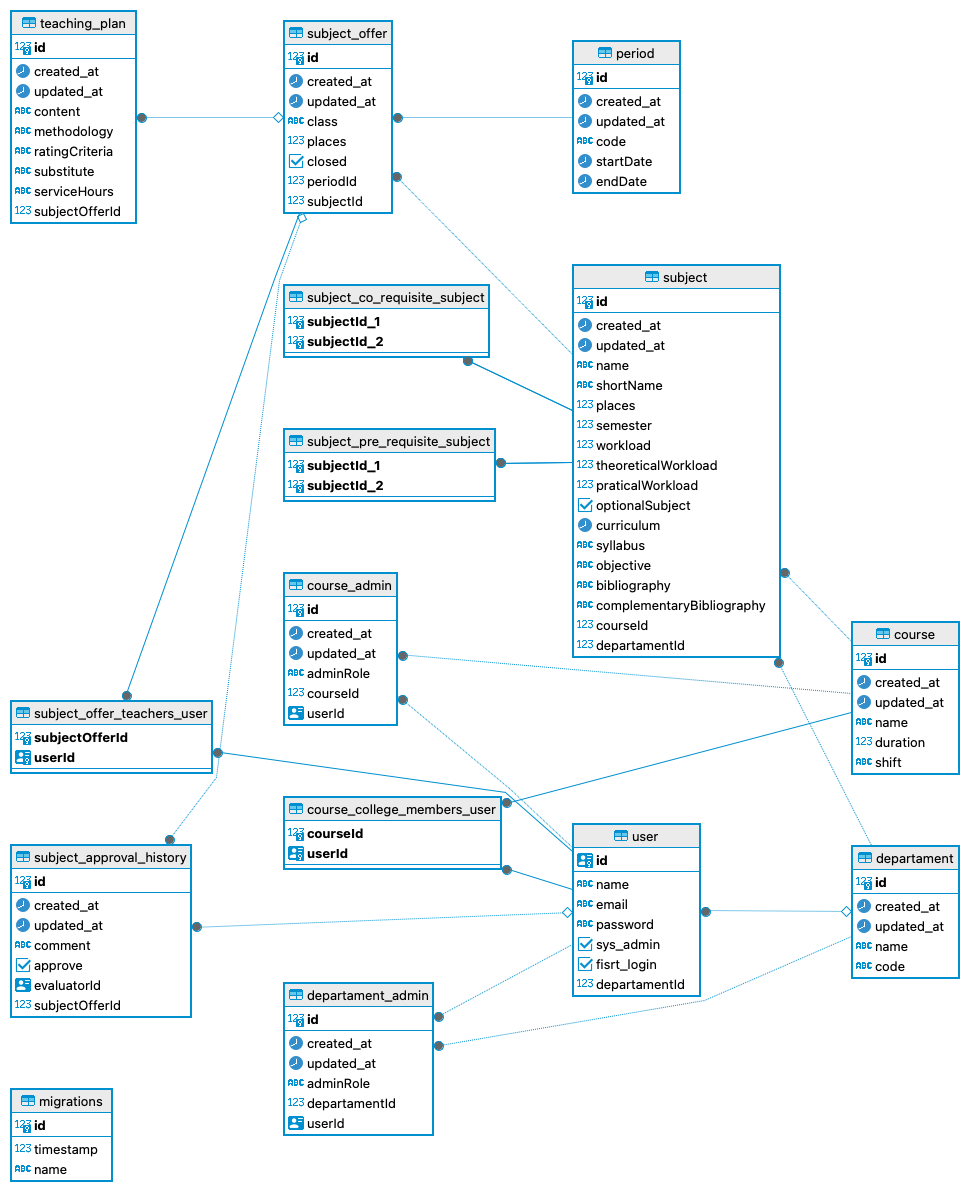
\includegraphics[width=350px]{imgs/model_db.png}
    \caption{Modelagem Banco de Dados.}
    \label{fig:Figura2}
\end{figure}

Foi escolhido o PostgreSQL como sistema gerenciador de banco de dados. Sua escolha se deu por ser um SGBD robusto e de código aberto. A construção foi feita com o auxilio do TypeORM, biblioteca que assiste nas operações junto ao banco de dados, abstraindo complexidades e trabalhando de forma orientada a objetos.


\section{Arquitetura do Sistema}

Conforme as necessidades identificadas, o sistema foi estruturado nas seguintes componentes: uma camada de frontend, que é voltada para o usuário final e tem como função exibir a interface gráfica, além de permitir a interação direta com o usuário; uma camada de backend, responsável pelo processamento das requisições recebidas do frontend, pela interação com o banco de dados, pela execução da lógica de negócios, pela validação e manipulação de dados, bem como pelo envio de respostas ao frontend; e, por fim, uma camada de banco de dados, onde os dados da aplicação são armazenados, recuperados e manipulados. Essa arquitetura é representada na Figura \ref{fig:DigImpl}.

\begin{figure}[h]
    \centering
    \includegraphics[scale=0.8]{imgs/diagrama_implantacao.png}
    \caption{Diagrama de Implantação.}
    \label{fig:DigImpl}
\end{figure}



Dentre as diversas bibliotecas e implementações presentes no sistema, destacam-se aquelas que desempenham um papel fundamental em sua caracterização e funcionamento. O cliente utiliza Next.js\footnote{https://nextjs.org}, com o suporte do Ant Design\footnote{https://ant.design}  e Styled Components\footnote{https://styled-components.com} para a criação e estilização das interfaces de usuário. A comunicação entre o frontend e o backend é realizada através do Axios\footnote{https://axios-http.com/ptbr/docs/intro}, responsável por efetuar as requisições HTTP. O backend, por sua vez, foi desenvolvido utilizando Express.js\footnote{https://expressjs.com/pt-br} e faz uso do TypeORM\footnote{https://typeorm.io/} para o gerenciamento das consultas ao banco de dados.


O fluxo de comunicação entre essas camadas pode ser descrito da seguinte forma:

\begin{enumerate}
    \item Requisição do Usuário: O usuário interage com a interface do frontend (por exemplo, clicando em um botão de "Salvar").
    \item Requisição HTTP: O frontend captura essa interação e envia uma requisição HTTP ao backend, especificando o tipo de ação a ser realizada (como salvar um novo registro no banco de dados).
    \item Processamento no Backend: O backend recebe a requisição, valida os dados recebidos, e se necessário, realiza operações de leitura ou escrita no banco de dados.
    \item Interação com o Banco de Dados: O backend se comunica com o banco de dados para armazenar, recuperar ou manipular dados conforme solicitado.
    \item Resposta ao Frontend: Após processar a requisição, o backend envia uma resposta de volta ao frontend. Essa resposta pode incluir dados (como uma lista de registros) ou uma confirmação de que a operação foi bem-sucedida.
    \item Atualização da Interface: O frontend recebe a resposta e, com base nos dados retornados, atualiza a interface do usuário, exibindo novas informações ou notificações conforme necessário.
\end{enumerate}

Para o lançamento da aplicação foi utilizado a Vercel\footnote{https://vercel.com}, que fornece ferramentas de desenvolvedor e infraestrutura em nuvem para construir, dimensionar e proteger serviços web. Nessa etapa foi utilizado os serviços em nuvem da plataforma, onde foi disponibilizado os componentes do sistema para a internet.


% diagrama de implantação
% explicando comunicação
% comunicação
% cada parte
% componentes do sistema
% deploy
% serviço de banco
% fluxo de dados
% sermaias abstrado citar sem necessariamente sem mostrar codigo





\section{Construção do Sistema}

Nesta sessão, será detalhado como cada componente discutido neste capítulo contribui para a construção do sistema. Nas Sessões \ref{subsec:constr:admin} a \ref{subsec:constr:professor}, são apresentadas as telas e os código dos casos de uso do sistema.


\subsection{Funcionalidades Geral e Administrativa} \label{subsec:constr:admin}

Nesta Sessão, serão apresentadas as telas comuns a todos os usuários do sistema e também as do usuário administrador.

\subsubsection{Cadastro de Usuário e Login}
Ao acessar o sistema, a primeira página apresentada ao usuário é a de Login (CDU01), seguida pela de Registro (CDU2). Nestes primeiros componentes do sistema, o que se destaca são a criação do modelo de usuário (Listagem \ref{list:UserModel}), representando a estrutura do dado presente no banco de dados em notação orientada a objeto, o mecanismo utilizando para criação de usuários, armazenamento de senhas e login no sistema, além da própria interface.


\begin{figure}[H]
    \centering
    \begin{subfigure}[h]{0.49\textwidth}
        \centering
        \includegraphics[scale=0.14]{imgs/login.png}
        \caption{Tela de Login}
        \label{fig:card}
    \end{subfigure}
    \begin{subfigure}[h]{0.49\textwidth}
        \centering
        \includegraphics[scale=0.14]{imgs/registro.png}
        \caption{Tela de registro}
        \label{fig:ccard1}
    \end{subfigure}
     \caption{Telas de Login e Registro}
    \label{fig:criacao:curso:dpto}
\end{figure}

% \begin{figure}[h]
%     \centering
%     \includegraphics[scale=0.3]{imgs/login.png}
%     \caption{Tela de Login.}
%     \label{fig:Login}
% \end{figure}

% \begin{figure}[h]
%     \centering
%     \includegraphics[scale=0.3]{imgs/registro.png}
%     \caption{Tela de Registro.}
%     \label{fig:Registro}
% \end{figure}


Na Listagem {\ref{list:UserModel}} apresentada, é possível observar a utilização do TypeORM, onde são descritas cada uma das propriedades do modelo de usuário e suas respectivas relações. A classe resultante possibilita a manipulação dos usuários no código, e, por meio das funcionalidades fornecidas pela biblioteca, permite a interação com o banco de dados.

\begin{listing}[h]
    \begin{minted}[linenos, bgcolor=lightgray, fontsize=\footnotesize]{typescript}
@Entity("user")
class User {
  @PrimaryGeneratedColumn("uuid")
  id!: string;

  @IsNotEmpty()
  @IsString()
  @Column({
    length: 128,
  })
  name!: string;
  
  @IsNotEmpty()
  @IsString()
  @Column({
    length: 256,
    select: false,
  })
  password!: string;
}
    \end{minted}
    \caption {Modelo de Usuário.}
    \label{list:UserModel}
\end{listing}

Para o registro do usuário, destacamos as principais validações cujas são a unicidade do e-mail fornecido \ref{list:registroCDU}, esta caso falhe apresenta retorna um erro ao usuário e a criptografia baseada em \textit{Hash} para armazenamento seguro da senha dos usuários.

\newpage

\begin{listing}[h]
    \begin{minted}[linenos, bgcolor=lightgray]{typescript}
const user = await this.repository.findOne(email, "email");

if (user) {
  Logger.error("validation failed.");
  throw new DuplicatedEntityError("Email already in use!");
}

const newUserData = {
  name,
  email,
  password: bcrypt.hashSync(password, 10),
};
    \end{minted}
    \caption{Registro de Usuário.}
    \label{list:registroCDU}
\end{listing}


lorem

\begin{listing}[h]
    \begin{minted}[linenos, bgcolor=lightgray]{typescript}
const user = (await this.repository.findOne(email, "email")) as User;

if (!user) {
  const message = "User not found";
  Logger.info(message);
  throw new AuthenticateFailError(message);
}

const { password: userPassword } = 
    (await this.repository.getUserPassword(user.id)) as User;

const userRoles = this._getUserRoles(user);

if (await bcrypt.compare(password, userPassword)) {
  const token = jwt.sign(
    { id: user.id, userRoles: userRoles },
    process.env.JWT_TOKEN as string,
    {
      expiresIn: process.env.JWT_EXPIRE,
    }
  );

  const resData = {
    id: user.id,
    name: user.name,
    email: user.email,
    roles: userRoles,
    token,
  };

  return resData;
}
    \end{minted}
    \caption{Login.}
    \label{list:login}
\end{listing}


\subsubsection{Painel Geral e Minha Conta}

O Painel Geral da aplicação é apresentado conforme a Figura \ref{fig:dashboard:mark}. É possível visualizar todos os módulos no menu principal localizado no topo da tela, os quais serão abordados em detalhes nas seções correspondentes a cada funcionalidade. Nesta etapa, destacamos a estrutura da interface da aplicação, ressaltando o uso do \textit{framework} React, no qual cada pequena estrutura é denominada "Componente". Esses componentes são reutilizados ao longo das diferentes páginas, variando apenas os dados exibidos. De forma geral a aplicação é estruturada com um componente \textit{Header}, destacado em vermelho na Figura \ref{fig:dashboard:mark}, ao qual agrupa os módulos e fornece o roteamento entre os mesmos, reúne funcionalidades que necessitam fácil manuseio como sair do sistema e a troca de período. Um \textit{Sider}, em amarelo, que apresenta listagens e navegabilidade em funcionalidades especificas ao módulo, e por fim um \textit{Content}, representado na figura em azul, este responsável por apresentar as informações e ações do sistema.

Minha Conta é a primeira página apresentada ao usuário ao fazer o login no sistema. Neste módulo possibilita-se a manutenção de conta permitindo funcionalidades como troca de senha e e-mail. Para tal função é utilizado um formulário para coletar as informações fornecidas pelo usuário (Listagem \ref{list:email}).

\begin{listing}[!h]
    \begin{minted}[linenos, bgcolor=lightgray]{java}
 <PageContent>
      <SForm
        form={form}
        name="basic"
        layout="vertical"
        initialValues={{ remember: true }}
        onFinish={handleSubmit}
        onFinishFailed={onFinishFailed}
        autoComplete="off"
      >
        <Form.Item
          label="Senha"
          name="password"
          rules={[
            {
              required: true,
              message: "Por favor insira sua senha atual!",
            },
          ]}
        >
          <Input.Password placeholder="Insira sua senha atual" />
        </Form.Item>
        <Form.Item
          label="Novo Email"
          labelAlign="left"
          name="email"
          rules={[
            {
              required: true,
              type: "email",
              message: "Insira um email válido",
            },
          ]}
        >
          <Input placeholder="Insira seu novo email" />
        </Form.Item>
        <Form.Item>
          <div style={{ display: "flex" }}>
            <Button type="primary" htmlType="submit">
              Confirmar
            </Button>
          </div>
        </Form.Item>
      </SForm>
</PageContent>
    \end{minted}
    \caption{Formulário troca de e-mail.}
    \label{list:email}
\end{listing}



\begin{figure}[h]
    \centering
    \includegraphics[scale=0.23]{imgs/pagina-minha-conta.png}
    \caption{Minha Conta e principais Componentes da interface.}
    \label{fig:dashboard:mark}
\end{figure}



\subsubsection{Pagina de Período}\label{subsec:pag-periodo}

Nesta página (\ref{fig:periodo}), o administrador tem a capacidade de criar períodos que serão utilizados na aplicação. No \textit{Sider}, são listados os períodos já criados, os quais podem ser selecionados para exibição de suas informações no \textit{Content}. Destaca-se nesta página o uso de listagem infinita, apresentado na Listagem \ref{list:listagem-infinita} que realizará a paginação automática à medida que o usuário navega pelos períodos criados. O código dessa listagem apresenta o componente React responsável por esse comportamento, onde podemos verificar as propriedades fornecidas ao componente que indicam o funcionamento da listagem infinita, onde tem-se a função \textit{LoadMoreData} responsável pela busca de novos itens e a propriedade \textit{hasMore} como variável de controle sob a necessidade da busca dos mesmos.


\begin{listing}[h]
    \begin{minted}[linenos, bgcolor=lightgray]{bash}
<InfiniteScroll
          dataLength={data.length}
          next={loadMoreData}
          hasMore={data.length < total}
          loader={<Skeleton avatar paragraph={{ rows: 1 }} active />}
          endMessage={<Divider plain>Não há mais itens! </Divider>}
          scrollableTarget="scrollableDiv"
>
    <AlternateList
        itemLayout="vertical"
        dataSource={data}
        locale={{
          emptyText: (
            <Empty
              image={Empty.PRESENTED_IMAGE_SIMPLE}
              description={false}
            />
          ),
        }}
        renderItem={(item: IPeriod) => (
          <List.Item>
            <Link href={`/dashboard/periods/${item.id}`}>
              <Card
                className={
                  Number(pId) === item.id ? "selected" : "notSelected"
                }
                hoverable
              >{`Periodo: ${item.code}`}</Card>
            </Link>
          </List.Item>
        )}
      />
</InfiniteScroll>
    \end{minted}
    \caption{Código listagem infinita.}
    \label{list:listagem-infinita}
\end{listing}


\begin{figure}[h]
    \centering
    \includegraphics[scale=0.23]{imgs/periodo.png}
    \caption{Página Período}
    \label{fig:periodo}
\end{figure}



\newpage

\subsubsection{Paginas de Curso e de Departamento}

Nessas páginas o sistema permite a criação e manutenção dos Departamentos e Cursos. Para o usuário administrador, responsável pela criação dos mesmos, é apresentado a opção de criação, demonstrada na Figura \ref{fig:tela:curso}, acima da listagem dos respectivos registros que seguem a mesma logica apresentada na Sessão \ref{subsec:pag-periodo}. Ao selecionar a opção será disponibilizado ao usuário os devidos formulários (Figura \ref{fig:criacao:curso:dpto}), estes deverão ser preenchidos com as informações necessárias para criação de cada registro. A Listagem \ref{list:insert-curso} apresenta o código relacionado a inserção dos dados no banco de dados, onde é possível visualizar como as operações de inserção são realizadas pelo TypeORM, sendo realizada a partir de métodos do repositório fornecido pela biblioteca.

\begin{figure}[h]
    \centering
    \includegraphics[scale=0.23]{imgs/tela-curso.png}
    \caption{Página Curso}
    \label{fig:tela:curso}
\end{figure}


\begin{figure}[h]
    \centering
    \begin{subfigure}[h]{0.4\textwidth}
        \centering
        \includegraphics[scale=0.23]{imgs/criar-curso.png}
        \caption{Formulário criação de Curso.}
        \label{fig:card}
    \end{subfigure}
    \begin{subfigure}[h]{0.4\textwidth}
        \centering
        \includegraphics[scale=0.23]{imgs/criar-departemento.png}
        \caption{Formulário criação de Departamento}
        \label{fig:ccard1}
    \end{subfigure}
     \caption{Formulários de criação de curso e departamento}
    \label{fig:criacao:curso:dpto}
\end{figure}


\begin{listing}[h]
    \begin{minted}[linenos, bgcolor=lightgray]{bash}
async save(data: Course) {
    const repository = getRepository(Course);

    if (data.admins && data.admins.length) {
      data.admins.forEach((admin) => {
        admin.createdAt = new Date();
      });
    }

    return repository.save(data);
}
    \end{minted}
    \caption{Código inserção de curso.}
    \label{list:insert-curso}
\end{listing}



\subsection{Funcionalidades do Curso} \label{subsec:constr:curso}


Após a criação de um curso pelo Administrador, o usuário designado como Coordenador do Curso receberá automaticamente o papel de Administrador de Curso no sistema, com base no vínculo estabelecido. Dessa forma, o Coordenador assumirá a responsabilidade de gerenciar os cursos a ele associados. Nesta Sessão, serão apresentadas as funcionalidades disponíveis nesse módulo.

Ao selecionar um curso, as respectivas informações serão exibidas no \textit{Content} da página, conforme ilustrado na Figura \ref{fig:tela:curso}. Logo acima dessas informações, encontra-se um menu de navegação que disponibiliza todas as funcionalidades relacionadas ao curso, tais como Disciplina, Colegiado, Oferta e Avaliações de Plano. O código apresentado na Listagem \ref{list:nav:curso} demostra como os itens da navegação são gerenciados.


\begin{listing}[h]
    \begin{minted}[linenos, bgcolor=lightgray]{bash}
function CoursesPage(props: CoursePageProps) {
  const { course } = props;

  const items = [
    {
      label: (
        <span>
          <InfoCircleOutlined /> Informações
        </span>
      ),
      key: "item-1",
      children: <CourseInfo courseInfo={course} />,
    },
  ];

  return (
    <PageContent>
      <Tabs
        defaultActiveKey="item-1"
        centered
        style={{ width: "100%" }}
        items={items}
      />
    </PageContent>
  );
}
    \end{minted}
    \caption{Código navegação conteúdo do Curso.}
    \label{list:nav:curso}
\end{listing}


\subsubsection{Disciplinas}

Essa página (\ref{fig:disciplina:curso}) permite a visualização e o gerenciamento das disciplinas do curso selecionado, utilizando um componente denominado \textit{Collapse}. Esse componente exibe uma lista de painéis inicialmente recolhidos, possibilitando sua expansão para a apresentação completa dos registros correspondentes.


\begin{figure}[h]
    \centering
    \includegraphics[scale=0.27]{imgs/disciplina-curso.png}
    \caption{Disciplinas do Curso}
    \label{fig:disciplina:curso}
\end{figure}

\subsubsection{Colegiado}

Com o objetivo de vincular usuários ao colegiado, um formulário é exibido acima da lista de usuários já cadastrados, conforme demonstrado na Figura \ref{fig:colegiado:curso}. Conforme exemplificado na Sessão \ref{subsec:constr:curso}, uma vez vinculado a um curso, o usuário recebe o nível de acesso de Membro do Colegiado na aplicação, sendo concedidos os acessos correspondentes.


\begin{figure}[h]
    \centering
    \includegraphics[scale=0.25]{imgs/colegiado-curso.png}
    \caption{Membros do Colegiado do Curso}
    \label{fig:colegiado:curso}
\end{figure}



\subsubsection{Ofertas do curso} \label{subsec:oferta:curso}

A página Ofertas do Curso (Figura \ref{fig:oferta:curso}) é projetada para o gerenciamento das ofertas de disciplinas vinculadas a um curso, que serão submetidas ao Departamento responsável. O usuário pode optar por ofertar todas as disciplinas do curso de forma simultânea (Figura \ref{fig:oferta:curso1}), com a possibilidade de definir se deseja ofertar apenas as disciplinas obrigatórias, apenas as opcionais, ou ambas. Esse recurso permite a criação de ofertas em larga escala, otimizando o tempo e garantindo a disponibilidade das disciplinas conforme as necessidades curriculares. Ao utilizar essa funcionalidade, o Sistema irá pressupor que as disciplinas serão de turma única, que poderá ser alterado posteriormente. Como alternativa, a página oferece a opção de ofertar disciplinas individualmente (Figura \ref{fig:oferta:curso2}), permitindo que o usuário especifique o numero de vagas e o nome da turma para cada disciplina, possibilitando a criação de mais de uma turma de uma disciplina por semestre. Após a criação de uma oferta, esta estará imediatamente disponível ao Departamento para que seja realizado o cadastro dos professores responsáveis pela ministração da disciplina. Para fins de formalização, a página dispõe de uma funcionalidade que permite a geração automática de um texto de solicitação ao Departamento, contendo todas as ofertas criadas e requisitando oficialmente a disponibilização das disciplinas correspondentes, conforme apresentado na Figura \ref{fig:text:dpto}. Além disso, a interface apresenta uma tabela com todas as ofertas cadastradas, exibindo informações como o nome da disciplina, o tipo (obrigatória ou opcional), numero de vagas, semestre, o nome da turma e os professores vinculados após o processo do Departamento.


\begin{figure}[h]
    \centering
    \includegraphics[scale=0.25]{imgs/ofertas-curso.png}
    \caption{Ofertas do Curso}
    \label{fig:oferta:curso}
\end{figure}


\begin{figure}[h]
    \centering
    \includegraphics[scale=0.25]{imgs/texto-curso.png}
    \caption{Texto gerado para envio ao departamento}
    \label{fig:text:dpto}
\end{figure}


\begin{figure}[h]
    \centering
     \begin{subfigure}[h]{0.4\textwidth}
        \centering
        \includegraphics[scale=0.30]{imgs/adc-oferta-bulk.png}
        \caption{Formulário criação de oferta em massa}
        \label{fig:oferta:curso1}
    \end{subfigure}
    \begin{subfigure}[h]{0.4\textwidth}
        \centering
        \includegraphics[scale=0.30]{imgs/adc-oferta-unica.png}
        \caption{Formulário criação de oferta única}
        \label{fig:oferta:curso2}
    \end{subfigure}
    \caption{Formulários de ofertas}
    \label{fig:oferta:curso-group}
\end{figure}


\begin{listing}[h]
    \begin{minted}[linenos, bgcolor=lightgray]{bash}
const alreadyExistingSubjects =
      await this.subjectOfferRepository.findExistentBulkSubject(
        courseId,
        periodId,
        addRequired,
        addOptional
      );

    const alreadyExistingSubjectsIDs = alreadyExistingSubjects.map(
      (e) => e.subject.id
    );

    const nonExistentSubject = courseSubjects.filter(
      (e) => !alreadyExistingSubjectsIDs.includes(e.id)
    );

    const requiredSubjectOffersData = nonExistentSubject
        .map((eachSubject) => {
          return Object.assign(new SubjectOffer(), {
            period: {
              id: periodId,
            },
            subject: {
              id: eachSubject.id,
            },
            places: eachSubject.places,
      });
});
    \end{minted}
    \caption{Código criação de ofertas em pacote}
    \label{list:bulk:create}
\end{listing}


O código apresentado na Listagem \ref{list:bulk:create} ilustra o procedimento de criação de ofertas em lote. Inicialmente, realiza-se uma busca pelas disciplinas selecionadas, sejam elas opcionais ou obrigatórias, seguida por uma filtragem das disciplinas já cadastradas, evitando-se, assim, duplicidades. Em seguida, a operação de salvamento em lote é executada no banco de dados por meio do repositório.

\subsubsection{Avaliação de Planos de Ensino}

A página tem como objetivo apresentar os planos de ensino preenchidos pelo professor, conforme descrito na Sessão \ref{subsec:constr:professor}, para avaliação pelos Membros do Colegiado. Nessa página, é exibida uma lista de disciplinas cujos planos já foram preenchidos. Ao selecionar uma disciplina, o respectivo plano é apresentado ao usuário, juntamente com as opções de aprovar ou rejeitar \ref{fig:avaliacao:plano}. No caso de rejeição, é necessário fornecer uma justificativa para concluir a ação.

% \begin{figure}[h]
%     \centering
%     \includegraphics[scale=0.25]{imgs/avaliação.png}
%     \caption{Tela avaliação de plano}
%     \label{fig:avaliacao:plano}
% \end{figure}



\subsection{Funcionalidades do Departamento} \label{subsec:constr:departamento}

As funcionalidades do Departamento \ref{fig:departamento} assemelham-se amplamente às apresentadas para o Curso na Sessão \ref{subsec:constr:curso}. Assim como ocorre no caso do Curso, ao ser criado, o Departamento passa a ser gerido pelo Chefe do Departamento indicado no momento de sua criação, a quem são atribuídas permissões de Administrador de Departamento no sistema. As semelhanças estendem-se também às telas de "Informação" e "Professores", que operam de maneira análoga às seções Informações e Membros do Colegiado do Curso, porém exibindo dados específicos do Departamento selecionado e oferecendo a funcionalidade de adicionar professores que poderão solicitar a ministração das ofertas criadas pelo Curso. Destaca-se ainda que, de forma semelhante ao Administrador de Curso e ao Administrador de Departamento, ao vincular um professor ao Departamento, este receberá automaticamente as permissões de professor no sistema, decorrentes do vínculo estabelecido.

% \begin{figure}[h]
%     \centering
%     \includegraphics[scale=0.25]{imgs/content-departamento.png}
%     \caption{Conteúdo do Departamento}
%     \label{fig:departamento}
% \end{figure}

\subsubsection{Encargos}\label{subsec:dpto:encargos}

Esta tela é responsável pelo gerenciamento dos encargos semestrais do Departamento. Nela são listados todos os encargos relativos às disciplinas ofertadas pelos cursos, bem como suas respectivas informações. Nessa fase, espera-se que os professores se candidatem para ministrar as disciplinas; uma vez que manifestem interesse, suas solicitações serão exibidas na lista conforme demonstrado na Figura \ref{fig:encardo:dpto}. O Chefe do Departamento possui a prerrogativa de excluir solicitações, permitindo a seleção final do professor. Após a escolha, o Chefe pode bloquear qualquer edição adicional por parte dos professores, utilizando o ícone localizado acima da listagem. Por fim, a tela oferece a opção de gerar uma mensagem para oficializar a seleção dos professores ao curso, recurso semelhante ao apresentado para o curso na Sessão \ref{subsec:oferta:curso}, a Listagem \ref{list:text:curse} demonstra como o texto é gerado a partir das ofertas e professores selecionados.


% \begin{figure}[h]
%     \centering
%     \includegraphics[scale=0.25]{imgs/encargos.png}
%     \caption{Encargos do departamento}
%     \label{fig:encardo:dpto}
% \end{figure}


\begin{listing}[h]
    \begin{minted}[linenos, bgcolor=lightgray]{bash}
<div>
    {offersByCourse && selectedCourse && (
      <div>
        {`Prezado(a) Coordenador(a), ${
          offersByCourse[selectedCourse].course.admins.find(
            (e) => e.adminRole === CourseAdminRole.COORDINATOR
          ).user.name
        }`}
        {offersByCourse[selectedCourse]?.offers.map((e, idx) => (
          <>
            <br />
            <br />
            <span>
              {`O(s) professor(es) ${e.teachers
                .map((eachTeacher) => eachTeacher.name)
                .join(", ")} lecionará(ão) a disciplina ${
                e.subject.name
              }, CH ${
                e.subject.workload
              }, para o curso ${selectedCourse}. Contato ${
                e.teachers.length > 1
                  ? "dos(as) professores(as)"
                  : "do(a) professor(a)"
              }
              : ${e.teachers.map((each) => each.email).join(", ")}`}
            </span>
          </>
        ))}
        <br />
        <br />
        Atenciosamente,
        <br />
        {user.name}
</div>    
    \end{minted}
    \caption{Código geração de mensagem para Curso}
    \label{list:text:curse}
\end{listing}


\subsection{Funcionalidades do Professor} \label{subsec:constr:professor}

Ao acessar o sistema, o usuário com perfil de Professor terá acesso aos módulos de Departamento e Minhas Disciplinas. Conforme apresentado na Seção \ref{subsec:dpto:encargos}, o Professor poderá se candidatar para ministrar disciplinas, sendo-lhe apresentada uma opção de vínculo ao acessar a tela de Encargos do Departamento. A Figura \ref{fig:prof:encargo} ilustra este comportamento. Após o encerramento das edições realizado pelo Chefe de Departamento, as disciplinas atribuídas aos professores serão exibidas no módulo Minhas Disciplinas. Nessa etapa, o professor torna-se responsável pelo preenchimento dos planos de ensino, que serão posteriormente submetidos à aprovação dos membros do colegiado. Conforme ilustrado na Figura \ref{fig:prof:minhas}, ao selecionar uma disciplina, o professor poderá associar seu plano de ensino à oferta correspondente.

% \begin{figure}[h]
%     \centering
%     \includegraphics[scale=0.25]{imgs/professor-encargo.png}
%     \caption{Vinculo professor e encargo}
%     \label{fig:prof:encargo}
% \end{figure}


% \begin{figure}[h]
%     \centering
%     \includegraphics[scale=0.25]{imgs/tela-professor.png}
%     \caption{Modulo Minhas Disciplinas}
%     \label{fig:prof:minhas}
% \end{figure}


\newpage
\section{Avaliação do Sistema}\label{ref:avaliação}

Para avaliar se o trabalho alcançou os objetivos apresentados no Capitulo \ref{cap:intro}, foi proposta uma análise do sistema desenvolvido, realizada por usuários que poderiam utilizá-lo em suas atividades semestrais. Para esse propósito, foi inicialmente elaborado um breve tutorial apresentando o sistema e suas funcionalidades por meio de vídeos. A estratégia adotada consistiu na criação de filmagens segmentadas de acordo com os diferentes perfis de usuários, considerando suas respectivas funções.

Esses vídeos foram compartilhados com o secretário do curso de Ciência da Computação da Universidade Federal de São João del Rei, bem como com a secretária do Departamento do mesmo curso e instituição. Além disso, foram disponibilizados usuários fictícios e uma base de dados de teste, permitindo que os participantes experimentassem as funcionalidades do sistema e compreendessem como ele poderia ser utilizado em suas atividades.

Por fim, para fins de avaliação, foi disponibilizado um questionário com as seguintes afirmações:

\begin{itemize}
    \item Eu acho que gostaria de usar esse sistema com frequência.
    \item Eu acho o sistema desnecessariamente complexo.
    \item Eu acho que precisaria de ajuda de uma pessoa com conhecimentos técnicos para usar o sistema.
    \item Eu acho que as várias funções do sistema estão muito bem integradas.
    \item Eu acho que o sistema apresenta muita inconsistência.
    \item Eu imagino que as pessoas aprenderão como usar esse sistema rapidamente.
    \item Eu achei o sistema atrapalhado de usar.
    \item Eu precisei aprender várias coisas novas antes de conseguir usar o sistema.
    \item Você acha que o sistema fez você cumprir suas atividades mais rapidamente?
    \item Você acha que o sistema ajuda ou atrapalha a cumprir suas atividades?
\end{itemize}

Para cada afirmação, foi estabelecida uma escala de respostas de 1 a 10, em que 1 corresponde a "Discordo Totalmente" e 10 a "Concordo Totalmente". As únicas exceções foram as últimas duas perguntas, cuja resposta poderia ser escolhida entre as opções "Sim" ou "Não".

Por fim, foi incluída uma última pergunta aos usuários com o objetivo de coletar \textit{feedbacks} gerais e sugestões para possíveis implementações futuras. Nesse contexto, foi questionado: "Sentiu falta de alguma funcionalidade? Caso sim, qual?". A resposta para essa pergunta foi disponibilizada em formato de texto livre, permitindo que os usuários compartilhassem suas impressões e comentários sobre o sistema de forma espontânea.


\subsection{Resultados obtidos}\label{ref:avaliação}

Com base no questionário aplicado, foram obtidas as seguintes respostas.

\begin{table}[h]
\begin{tabular}{|l|c|}
\hline
\rowcolor[HTML]{96FFFB} 
Afirmação/Pergunta                                                                                                                       & \multicolumn{1}{l|}{\cellcolor[HTML]{96FFFB}Média das Respostas} \\ \hline
Eu acho que gostaria de usar esse sistema com frequência.                                                                                & 10                                                           \\ \hline
Eu acho o sistema desnecessariamente complexo.                                                                                           & 1                                                            \\ \hline
\begin{tabular}[c]{@{}l@{}}Eu acho que precisaria de ajuda de uma pessoa \\ com conhecimentos técnicos para usar o sistema.\end{tabular} & 1                                                            \\ \hline
\begin{tabular}[c]{@{}l@{}}Eu acho que as várias funções do sistema estão muito \\ bem integradas.\end{tabular}                          & 10                                                           \\ \hline
Eu acho que o sistema apresenta muita inconsistência.                                                                                    & 1                                                            \\ \hline
\begin{tabular}[c]{@{}l@{}}Eu imagino que as pessoas aprenderão como usar esse \\ sistema rapidamente.\end{tabular}                      & 10                                                           \\ \hline
Eu achei o sistema atrapalhado de usar.                                                                                                  & 1                                                            \\ \hline
\begin{tabular}[c]{@{}l@{}}Eu precisei aprender várias coisas novas antes de conseguir \\ usar o sistema.\end{tabular}                   & 1                                                            \\ \hline
\begin{tabular}[c]{@{}l@{}}Você acha que o sistema fez você cumprir suas atividades \\ mais rapidamente?\end{tabular}                    & 1 resposta Sim                                                          \\ \hline
\begin{tabular}[c]{@{}l@{}}Você acha que o sistema ajuda ou atrapalha a cumprir \\ suas atividades?\end{tabular}                         & 1 resposta Sim                                                          \\ \hline
\end{tabular}
\end{table}


Quanto à pergunta aberta "Sentiu falta de alguma funcionalidade? Em caso afirmativo, qual?", foi registrada a seguinte resposta:

\begin{quote}
O sistema quando testado por nós não estava com todas as funcionalidades, achei interessante e bem interativo o manuseio do mesmo. Foi feito os testes necessários e foi muito positivo. 

Em relação a essa pergunta "Você acha que o sistema ajuda ou atrapalha a cumprir suas atividades?". A resposta foi sim, mas acredito que deveria ser Ajuda ou atrapalha nas respostas. Na minha concepção o sistema agrega e ajuda aos trabalhos administrativos das coordenadorias de curso. \end{quote}

Nesse contexto, as funcionalidades que estavam ausentes foram implementadas na etapa final do trabalho, e os participantes dos testes foram convidados a avaliar a nova funcionalidade.

Assim, com base nos resultados obtidos a partir das respostas ao questionário, foi possível verificar que o software alcançou seus principais objetivos. As percepções dos usuários foram amplamente positivas, confirmando que se trata de uma solução com elevado nível de usabilidade e cujas funcionalidades efetivamente atenderam às necessidades do público-alvo.
% \include{chapters/05_results}
\chapter{Conclusão}\label{cap:conclusao}

Durante o desenvolvimento desde trabalho, foi possível constatar a complexidade e a extensão do processo semestral realizado pelas coordenações de curso. Nesse contexto, a implementação de sistemas informatizados assume um papel fundamental na modernização e otimização das atividades gerenciais, contribuindo para a melhoria da comunicação interna e externa entre os setores, a agilidade e padronização das tarefas, além de minimizar a ocorrência de retrabalhos.

\section{Contribuições}

O trabalho desenvolvido resultou em uma ferramenta que centraliza, de forma eficiente, o processo de registro de disciplinas e a alocação de encargos didáticos em um único sistema. Com isso, oferece suporte às coordenações de curso e departamentos na organização e no planejamento dos encargos didáticos a cada período letivo. Além disso, simplifica o processo de definição das disciplinas a serem ofertadas em cada período, proporcionando aos departamentos uma visão clara e detalhada de suas responsabilidades. Por fim, o sistema busca agilizar e otimizar a indicação de docentes para os encargos atribuídos, tornando esse processo mais eficiente e assertivo.


\section{Limitações}\label{sec:limitacoes}

Embora o trabalho apresentado tenha alcançado os objetivos propostos, durante o processo de desenvolvimento foram identificadas possíveis limitações em seu funcionamento. O estudo foi conduzido com foco específico na aplicação ao curso de Ciência da Computação da Universidade Federal de São João del Rei, o que pode resultar em restrições caso seja adaptado para outros cursos ou instituições. Contudo, o sistema foi projetado de maneira a ser flexível, permitindo futuras implementações e customizações relacionadas às suas regras de negócio.


\section{Trabalhos Futuros}

Por fim, com o objetivo de fomentar a continuidade deste estudo, foram sugeridas linhas de trabalho futuro, identificadas a partir das necessidades observadas durante a aplicação do sistema em situações reais.

Conforme apresentado na Sessão \ref{sec:limitacoes}, a possibilidade de novas implementações, considerando as demandas de outros cursos e instituições, constitui uma oportunidade para ampliar a escala e a abrangência do sistema.

Adicionalmente, a inclusão de módulos destinados ao gerenciamento de atividades como a elaboração de horários, considerando a disponibilidade de professores, e o planejamento do uso de salas e laboratórios, representa outro conjunto de funcionalidades semestrais que poderiam enriquecer o sistema. Tais melhorias, especialmente com a aplicação de técnicas de Inteligência Artificial, têm o potencial de tornar o software ainda mais robusto e completo.

% ----------------------------------------------------------
% -- POST-TEXTUAL ELEMENTS
% ----------------------------------------------------------
\postextual
\bookmarksetup{startatroot} % Resets bookmark hierarchy for post-textual elements

% --- Bibliography ---
% The 'abnt-num' style creates numeric citations. For author-date, use 'abnt-alf'.
\bibliographystyle{abnt-num}
% The .bib file containing your references
% [TODO: Add your references to the 'references.bib' file]
% \bibliography{references}

% --- Appendices (Optional) ---
% [TODO: Uncomment if you have appendices]
% \chapter*{Apêndices}
\hypertarget{apendices}{}  % Create the target for the hyperlink
\addunnumberedchapter[apendices]{Apêndices}

% Change section numbering to use letters
\renewcommand{\thesection}{\Alph{section}}

Content here...

\section{Primeiro Apêndice}
\section{Segundo Apêndice}
\section{Terceiro Apêndice}

% --- Attachments (Optional) ---
% [TODO: Uncomment if you have attachments]
% \chapter*{Anexos}
\hypertarget{anexos}{}  % Create the target for the hyperlink
\addunnumberedchapter[anexos]{Anexos}

% Change section numbering to use letters and restart from A
\setcounter{section}{0}
\renewcommand{\thesection}{\Alph{section}}

Content here...

\section{Primeiro Anexo}
\section{Segundo Anexo}
\section{Terceiro Anexo}

% --- Index (Optional) ---
% [TODO: Uncomment to print the remissive index]
% \printindex
% --- ADD THE CLOSING PAGE COMMAND HERE ---
\imprimirclosingpage
\end{document}